As an intermediate step, our compiler first transforms rules into high level
instructions that are then transformed into C++. In Appendix~\ref{appendix:vm}
we present an overview of the high level instructions that can be used as a
reference to the operations that are required by the compiler. In this section,
we present the main algorithm of the compiler and its key optimizations. To make
our presentation more readable, we present our examples using pseudo-code
instead of C++ code.

\subsection{Ordinary Rules}\label{sec:compile}

After an inference rule is compiled, it must respect the \emph{fact constraints}
(facts must exist in the database) and the \emph{join constraints} that can be
represented by variable constraints and/or boolean expressions. For instance,
consider the second rule of the bipartiteness checking program presented in
Fig.~\ref{language:code:bichecking}:

\begin{Verbatim}[fontsize=\codesize]
visit(A, P), colored(A, P) -o colored(A, P).
\end{Verbatim}

The fact constraints include the facts required to trigger the rule, namely
\code{visit(A, P)} and \code{visited(A, P)}, and the join constraints include
the implicit constraint that the second argument of \code{visit} must be equal
to the second argument of \code{colored} because the variable \code{P} is used
for both arguments. However, rules may also have explicit constraints, such as:

\begin{Verbatim}[fontsize=\codesize]
visit(A, P1), colored(A, P2), P1 <> P2 -o fail(A).
\end{Verbatim}

The data structures presented in Section~\ref{sec:data_structures} support
iteration over facts and for linear facts, they also support deletion. Iteration
is provided through \emph{iterators}. For linked lists, the iterator is simply
the fact that can be iterated by following the \code{next} pointers. For hash
tables, it is possible to iterate through the whole table or iterate through a
single bucket. For tries, while iteration goes through every fact, the operation
can be customized with a matching specification in order to prune search. A
matching specification includes argument assignments, such as, argument $i = V$,
where $V$ is a concrete value.  To illustrate how rules are compiled, consider
again the rule:

\begin{Verbatim}[fontsize=\codesize]
visit(A, P), colored(A, P) -o colored(A, P).
\end{Verbatim}

The compiler transforms the rule into two nested \emph{while} loops, as follows:

\begin{Verbatim}[numbers=left,fontsize=\codesize]
colored_list <- linked_list("colored")
visit_list <- linked_list("visit")
visit <- visit_list.head()
while(visit is valid)
{
   colored <- colored_list.head() // Retrieve first element of the list.
   while(colored is valid)
   {
      if(visit.get_int(1) == colored.get_int(1)) { // Equal arguments?
         new_colored <- create_fact("colored") // New fact for predicate colored.
         new_colored.set_int(1, visit.get_int(1)) // Set arguments.

         // New fact is derived.
         colored_list.add(new_colored) // Add new fact to the linked list.

         // Deleting facts.
         colored <- colored_list.erase_and_next(colored)
         visit <- visit_list.erase_and_next(visit)
         goto next
      }
      colored <- colored.next()
   }
   visit <- visit.next()
next:
   continue
}
\end{Verbatim}

The compilation algorithm iterates through the atomic propositions in rule's LHS
and creates nested loops to try all the possible combinations of facts.  For
this rule, all the pairs of facts \code{colored} and \code{visit} must be
matched until the implicit constraint is true. First, the \code{colored} linked
list is iterated over by first retrieving the head fact and then using the
\code{next} pointer of each fact. Inside this outer loop, a nested \code{while}
loop is created for predicate \code{visit}. This inner loop includes a check for
the constraint.

If the constraint expression is true then the rule matches and a new
\code{colored} fact is derived and two used linear facts are consumed by erasing
them from the linked lists. After the rule is derived, the \code{visit} and
\code{colored} facts are deleted from the linked list and the pointers adjusted
to the next elements of each list. Afterwards, the \code{goto next} statement is
used to jump to the outer loop, which will use the new fact pointers. This
forces the procedure to try all the combinations of the rule from the database.
Furthermore, we must jump to the first linear loop because we cannot use the
next fact from the deepest loop since we may have constraints between the first
linear loop and the deepest loop that were validated using deleted facts.

If the implicit constraint had failed, another \code{visit} fact would have been
used by assigning \code{visit} to \code{visit.next()}.  Likewise, if the initial
\code{colored} fact fails for all \code{visit} facts, then the next
\code{colored} fact in the list is tried by following the \code{next} pointer.

In order to understand how rule priorities affect compilation, consider a
slightly different bipartiteness checking program where the second and third
rules are swapped:

\begin{Verbatim}[numbers=left,fontsize=\codesize,commandchars=\*\[\]]
visit(A, P), uncolored(A)
   -o {B | !edge(A, B) -o visit(B, next(P))},
      colored(A, P).

visit(A, P1), colored(A, P2), P1 <> P2 -o fail(A).*label[line:implementation:higher]

*textbf[visit(A, P), colored(A, P) -o colored(A, P).]

visit(A, P), fail(A) -o fail(A).
\end{Verbatim}

The procedure for the rule being compiled cannot be the same since the derived
\code{colored} fact is used in the LHS of a higher priority rule, namely, the
rule in line~\ref{line:implementation:higher}. Once the \code{colored} fact is
derived, the procedure must return to schedule the higher priority rule, as
follows:

\begin{Verbatim}[numbers=left,fontsize=\codesize,commandchars=\$\#\&]
colored_list <- linked_list("colored")
visit_list <- linked_list("visit")
colored <- colored_list.head()
while(colored is valid)
{
   visit <- visit_list.head() // Retrieve first element of the list.
   while(visit is valid)
   {
      if(visit.get_int(1) == colored.get_int(1)) { // Equal arguments?
         new_colored <- create_fact("colored") // New fact for predicate colored.
         new_colored.set_int(1, visit.get_int(1)) // Set arguments.

         // New fact is derived.
         colored_list.add(new_colored) // Add new fact to the linked list.

         // Deleting facts.
         colored_list.erase_and_next(colored)
         visit_list.erase_and_next(visit)
         $textbf#return&
      }
      visit <- visit.next()
   }
   colored <- colored.next()
}
\end{Verbatim}

This enforces the priority semantics of the language. When a rule derives facts
that were used as input to a higher priority rule, the initial rule is only
derived once because the newly derived facts may trigger the derivation of a
higher priority rule.
    
\begin{figure}
\begin{algorithm}[H]
 \KwData{Rule R1, Rules}
 \KwResult{Compiled Code}
 $LHSProps \longleftarrow LHSAtomicPropositionsFromRule(R1)$\;
 $Constraints \longleftarrow ConstraintsFromRule(R1)$\;
 $Code \longleftarrow CreateFunctionForRule()$\;
 $FactIterators \longleftarrow []$\;
 $CompiledProps = []$\;
 \While{$LHSProps$ not empty}{
  $Prop \longleftarrow RemoveBestProposition(LHSProps)$\;
  $CompiledProps.push(Prop)$\;
  $Iterator \longleftarrow Code.InsertIteration(Prop)$\;
  $FactIterators.push(Iterator)$\;
  \tcc{Select constraints that are covered by CompiledFacts.}
  $NextConstraints \longleftarrow RemoveConstraints(Constraints, CompiledProps)$\;
  $Code.InsertConstraints(NextConstraints)$\;
 }
 $RHSProps = RHSAtomicPropositionsFromRule(R1)$\;
 \While{$RHSProps$ not empty}{
    $Prop \longleftarrow RemoveFact(RHSProps)$\;
    $Code.InsertDerivation(Prop)$\;
 }
 \For{$Iterator \in FactIterators$}{
    \If{$IsLinear(Iterator)$}{
       $Code.InsertRemove(Iterator)$\;
    }
 }
 \tcc{Enforce rule priorities.}
 \uIf{$FactsDerivedUsedBefore(Rules, R1)$}{
    $Code.InsertReturn()$\;
 }
 \Else{
    $Code.InsertGoto(FirstLinear(FactIterators))$\;
 }
 \Return{$Code$}
\end{algorithm}
 \caption{Compiling LM rules into C++ code.}
 \label{alg:compile_rule}
\end{figure}

Figure~\ref{alg:compile_rule} presents the algorithm for compiling rules into
C++ code. First, we split the rule's RHS into atomic propositions and
constraints. Fact expressions map directly to iterators while fact constraints
map to \emph{if} expressions. A possible compilation strategy is to first
compile all the atomic propositions and then compile the constraints. However,
this may require unneeded database lookups since some constraints may fail
early.  Therefore, our compiler introduces constraints as soon as all the
variables in the constraint are all included in the already compiled atomic
propositions. The order in which fact propositions are selected for compilation
does not interfere with the correctness of the compiled code, thus our compiler
selects the atomic proposition ($RemoveBestProposition$) by their potential to
activate constraints, therefore avoiding undesirable database lookups. If two
atomic propositions have the same number of new constraints, then the compiler
always picks the persistent proposition since persistent facts are not deleted.

Derivation of new facts belonging to the local node implies adding the new fact
to the local node data structure. Facts that belong to other nodes are sent
using an appropriate runtime API.

\subsection{Persistence Checking}

Not all linear facts need to be deleted. For instance, in the compiled rule
above, the fact \code{colored(A, P)} is re-derived in the rule's RHS.  Our
compiler is able to turn linear loops into persistent loops for linear facts
that are consumed and then asserted. The rule is then compiled as follows:

\begin{Verbatim}[numbers=left,fontsize=\codesize,commandchars=\$\#\&]
colored_list <- linked_list("colored")
visit_list <- linked_list("visit")
colored <- colored_list.head()
while(colored is valid)
{
   visit <- visit_list.head() // Retrieve first element of the list.
   while(visit is valid)
   {
      if(visit.get_int(1) == colored.get_int(1)) { // Equal arguments?
         // Delete visit.
         visit <- visit_list.erase_and_next(visit) // Get next visit fact.
         goto next$label#line:implementation:goto&
      }
      visit <- visit.next()
$textbf#next:&
      $textbf#continue&
   }
   colored <- colored.next()
}
\end{Verbatim}

In this new version of the code, only the \code{visit} facts are deleted, while
the \code{colored} facts remain untouched. In the bipartiteness checking
program, each node has one \code{colored} fact and this compiled code simply
filters out the \code{visit} facts with the same color. Please note that the
\code{colored} facts are now iterated in the outer loop in order to make the
\code{goto} statement jump to the inner loop. This is now possible because the
\code{colored} next is not deleted during rule derivation.

\subsection{Updating Facts}

Many inference rules consume and then derive the same predicate but with
different arguments. The compiler recognizes those cases and, instead of
consuming the fact from its linked list or hash table, it updates the fact
in-place. As an example, consider the following rule:

\begin{Verbatim}[fontsize=\codesize]
new-neighbor-pagerank(A, B, New),
neighbor-pagerank(A, B, Old)
   -o neighbor-pagerank(A, B, New).
\end{Verbatim}

Assuming that \code{neighbor-pagerank} is stored in a hash table and indexed by
the second argument, the code for the rule above is as follows:

\begin{Verbatim}[numbers=left,fontsize=\codesize]
new_neighbor_pagerank_list <- linked_list("new-neighbor-pagerank")
neighbor_pagerank_table <- hash_table("neighbor-pagerank")
new_neighbor_pagerank <- new_neighbor_pagerank.head()
while(new_neighbor_pagerank is valid)
{
   // Hash table for neighbor-pagerank is indexed by the second argument,
   // therefore we search for the bucket using the second argument of new-neighbor-pagerank.
   neighbor_pagerank <- neighbor_pagerank_table.lookup(new_neighbor_pagerank.get_node(1))
   while(neighbor_pagerank is valid)
   {
      if(new_neighbor_pagerank.get_node(1) == neighbor_pagerank.get_node(1))
      {
         // Update fact argument.
         neighbor_pagerank.set_float(2, new_neighbor_pagerank.get_float(2))
         new_neighbor_pagerank <- new_neighbor_pagerank_list.
                  erase_and_next(new_neighbor_pagerank)
         goto next
      }
      neighbor_pagerank <- neighbor_pagerank.next()
   }
   new_neighbor_pagerank <- new_neighbor_pagerank.next()
next:
   continue
}
\end{Verbatim}

Note that \code{neighbor-pagerank} fact is updated using \code{set\_float}. The
rule also does not return since it is the highest priority rule. If there was a
higher priority rule using \code{neighbor-pagerank}, then the code would have to
return since the act of updating a fact is equivalent to deriving a new one.

\subsection{Enforcing Linearity}

We have already introduced the \code{goto} statement as a way to avoid reusing
consumed linear facts. However, this is not enough in order to enforce
linearity of facts. Consider the following inference rule:

\begin{Verbatim}[fontsize=\codesize]
add(A, N1), add(A, N2) -o add(A, N1 + N2).
\end{Verbatim}

Using the standard compilation algorithm, two nested loops are created, one for
each \code{add} fact. However, notice that there is an implicit constraint when
creating the iterator for \code{add(A, N2)} since this fact cannot be the same
as the first one. That would invalidate linearity since a single linear fact
would be used to prove two linear facts. This is easily solved by adding a
constraint in the inner loop by checking if the second fact is the same as the
first one.

\begin{Verbatim}[numbers=left,fontsize=\codesize]
add_list <- linked_list("add")
add1 <- add_list.head()
while(add1 is valid)
{
   add2 <- add_list.head()
   while(add2 is valid)
   {
      if(add1 != add2)
      {
         add1.set_int(1, add1.get_int(1) + add2.get_int(1))
         add2 <- add_list.erase_and_next(add2)
         goto next
      }
      add2 <- add2.next()
   }
   add1 <- add1.next()
next:
   continue
}
\end{Verbatim}

Figure~\ref{fig:local:update_add} presents the steps for executing this rule
when the database contains three facts. The fact variables never point to the
same fact.

\begin{figure}
\centering
\begin{minipage}{.5\textwidth}
  \centering
  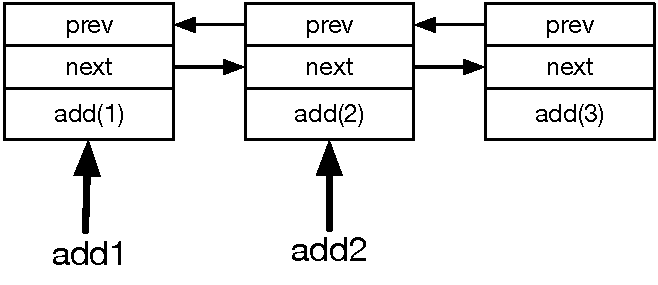
\includegraphics[width=.8\linewidth]{figures/compiler/update}
\end{minipage}%
\begin{minipage}{.5\textwidth}
  \centering
  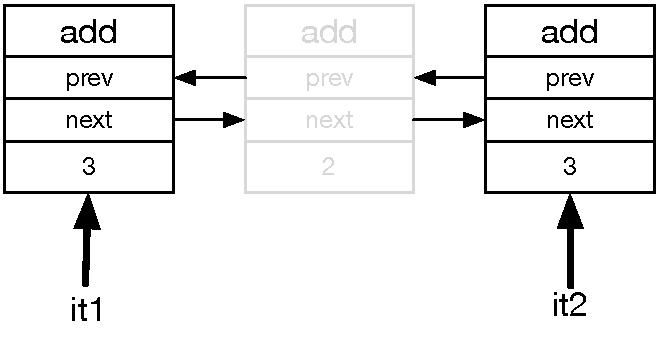
\includegraphics[width=0.8\linewidth]{figures/compiler/update2}
\end{minipage}
\begin{minipage}{.5\textwidth}
   \centering
   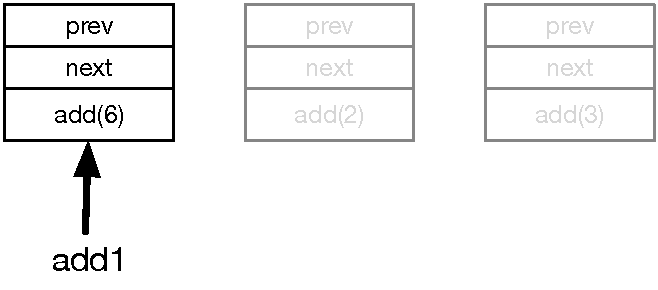
\includegraphics[width=0.8\linewidth]{figures/compiler/update3}
\end{minipage}
\caption{Executing the add rule. First, the two iterators point to
   the first and second facts and the former is updated while the latter is
   consumed. The second iterator then moves to the next fact and the first fact is
   updated again, now to the value \code{6}, the expected result.}
\label{fig:local:update_add}
\end{figure}

\subsection{Comprehensions}

Consider the comprehension used in the first rule of the bipartiteness checking
program in Fig.~\ref{language:code:bichecking}:

\begin{Verbatim}[fontsize=\codesize]
visit(A, P), uncolored(A)
   -o {B | !edge(A, B) -o visit(B, next(P))},
      colored(A, P).
\end{Verbatim}

The attentive reader will remember that comprehensions are sub-rules, therefore
they should be compiled like normal rules. Comprehensions must also derive all
possible combinations. However, the rule itself must return if any combination
of the comprehension has derived a fact that is used by a higher priority rule.
The example rule does not need to return since it has the highest priority and
the \code{visit} facts derived in the comprehension are contained in other
nodes. The code for the rule is shown below:

\begin{Verbatim}[numbers=left,fontsize=\codesize]
colored_list <- linked_list("colored")
visit_list <- linked_list("visit")
uncolored_list <- linked_list("uncolored")
visit <- visit_list.head()
while(visit is valid)
{
   uncolored <- uncolored_list.head()
   while(uncolored is valid)
   {
      // Comprehension code.
      edge_trie <- trie("edge")
      edge <- edge_trie.first()
      while(edge is valid)
      {
         new_visit <- create_fact("visit") // New visit fact.
         new_visit.set_int(1, next(visit.get_int(1)))
         // Send fact to B.
         send_fact(new_visit, edge.get_node(1))
         edge <- edge.next()
      }
      new_colored <- create_fact("colored")
      new_colored.set_int(1, visit.get_int(1))
      colored_list.add(new_colored)
      visit <- visit_list.erase_and_next(visit)
      uncolored <- uncolored_list.erase_and_next(uncolored)
      goto next
   }
   uncolored <- uncolored.next()
next:
   continue
}
\end{Verbatim}

Special care must be taken when the comprehension's sub-rule uses the same
predicates that are derived by the main rule. Rule inference must be atomic in
the sense that, after a rule matches, the comprehensions in the rule's RHS can
use the facts that were present before the rule was matched. Consider a rule
with $n$ comprehensions or aggregates, where $CLHS_i$ and $CRHS_i$ is the LHS
and RHS of the comprehension/aggregate, respectively, and $RHSP$ represents the
atomic propositions found in rule's RHS. The formula used by the compiler to
detect conflicts between predicates is the following:

\[
\bigcup^{n}_i[CLHS_i \cap RHSP] \cup \bigcup^{n}_i [CLHS_i \cap \bigcup^{n}_j[CRHS_j]]
\]

If the result of the formula is not empty, then the compiler disables
optimizations for the conflicting predicates and derives the corresponding facts
into the fact buffer that are then added back into the database. As an example,
consider the following rule:

\begin{Verbatim}[fontsize=\codesize]
update(A), !edge(A, B)
   -o {P | points(A, B, P) -o update(B)},
      points(A, B, 1).
\end{Verbatim}

We have $n = 1$ comprehensions, where $CLHS_0 = $ \code{points(A, B, P)},
$CRHS_0 =$ \code{update(B)}, and $RHSP = $ \code{points(A, B, 1)}. There is a
conflict because $CLHS_0 \cap RHSP = \{\mathtt{points}\}$, which requires
\code{points(A, B, 1)} to be derived after the comprehension or be stored in a
temporary data structure to avoid conflicts with the comprehensions, which could
consume the newly derived fact. Fortunately, most rules in LM programs do not
show these kinds of conflicts and thus can be fully optimized.

\subsection{Aggregates}

Aggregates are similar to comprehensions. They are also sub-rules but a value is
accumulated for each combination of the sub-rule. After all the combinations are
inferred, a final RHS term is derived with the accumulated term. Consider the
following rule that computes a PageRank value by aggregating all neighbors
PageRank values:

\begin{Verbatim}[fontsize=\codesize]
update(A), pagerank(A, OldRank)
      -o [sum => V; B | neighbor-pagerank(A, B, V) -o neighbor-pagerank(A, B, V)
            -> pagerank(A, damping/P + (1.0 - damping) * V)].
\end{Verbatim}

The variable \code{V} is initialized to \code{0.0} and sums all the PageRank
values of the neighbors as seen in the code below. The aggregate value is then
used to update the second argument of the initial \code{pagerank} fact.

\begin{Verbatim}[numbers=left,fontsize=\codesize]
pagerank_list <- linked_list("pagerank")
update_list <- linked_list("update")
neighbor_pagerank_list <- linked_list("neighbor_pagerank_list")
pagerank <- pagerank_list.head()
while(pagerank is valid)
{
   update <- update_list.head()
   while(update is valid)
   {
      V <- 0.0
      neighbor_pagerank <- neighbor_pagerank_list.head()
      while(neighbor_pagerank is valid)
      {
         V <- V + neighbor_pagerank.get_float(2)
         neighbor_pagerank <- neighbor_pagerank.next()
      }
      // RHS of the aggregate
      pagerank.set_float(1, damping / P + (1.0 - damping) * V)
      update <- update_list.erase_and_next(update)
      goto next
   }
   pagerank <- pagerank.next()
next:
   continue
}
\end{Verbatim}

